
\de{ĐỀ THI HỌC KỲ I NĂM HỌC 2022-2023}{THPT Bình Tân}
\begin{center}
	\textbf{PHẦN 1 - TRẮC NGHIỆM}
\end{center}
\Opensolutionfile{ans}[ans/ans]
%Câu 1...........................
\begin{ex}%[0T1Y1-3]%[Dự án đề kiểm tra NH22-23 - Huỳnh Quy]%[THPT Bình Tân]
	Cho mệnh đề $\forall x\in \mathbb{R}\colon x^3+x>0$. Phủ định mệnh đề này là
	\choice
	{$\exists x\in \mathbb{R}\colon x^3+x<0$}
	{\True $\exists x\in \mathbb{R}\colon x^3+x\leq 0$}
	{$\exists x\in \mathbb{R}\colon x^3+x=0$}
	{$\forall x\in \mathbb{R}\colon x^3+x\leq 0$}
	\loigiai{
	Mệnh đề phủ định của mệnh đề: ``$\forall x\in \mathbb{R}\colon x^3+x>0$'' là ``$\exists x\in \mathbb{R}\colon x^3+x\leq 0$''.
	}
\end{ex}

%Câu 2...........................
\begin{ex}%[0T3B1-1]%[Dự án đề kiểm tra NH22-23 - Huỳnh Quy]%[THPT Bình Tân]
	Cho hàm số $f(x)=\heva{
	&\dfrac{2\sqrt{x-2}-3}{x-1}&\quad\text{khi} \quad x\geq 2\\
	&x^2+2&\quad\text{khi}\quad x<2
	}$. Tính $P=f(2)+f(-2)$.
	\choice
	{\True $P=3$}
	{$P=2$}
	{$P=\dfrac{7}{2}$}
	{$P=6$}
	\loigiai{
	Ta có
	\begin{itemize}
		\item $f(2)=\dfrac{2\sqrt{2-2}-3}{2-1}=-3$.
		\item $f(-2)=(-2)^2+2=6$.
	\end{itemize}	
	Do đó $P=f(2)+f(-2)=-3+6=3$.
	}
\end{ex}

%Câu 3...........................
\begin{ex}%[0T3B2-1]%[Dự án đề kiểm tra NH22-23 - Huỳnh Quy]%[THPT Bình Tân]
	Cho hàm số bậc hai có bảng biến thiên như sau
	\begin{center}

\begin{tikzpicture}
\tkzTabInit[lgt=1.4,espcl=2.0,deltacl=.5,nocadre]
{$x$ /1, $y$ /1.7}
{$-\infty$ , $1$ , $+\infty$}
\tkzTabVar{-/$-\infty$ ,+/$21$  ,-/$-\infty$}
\end{tikzpicture}
\end{center}
Hàm số này nghịch biến trên
	\choice
	{\True $(1;+\infty)$}
	{$(-\infty;21)$}
	{$(-\infty;1)$}
	{$(-21;+\infty)$}
	\loigiai{
	Hàm số nghịch biến trên khoảng $(1;+\infty)$.	
	}
\end{ex}

%Câu 4...........................
\begin{ex}%[0T5Y4-1]%[Dự án đề kiểm tra NH22-23 - Huỳnh Quy]%[THPT Bình Tân]
	Cho hai vectơ tùy ý, khác $\overrightarrow{0}$. Khẳng định nào dưới đây \textbf{\textit{đúng}}?
	\choice
	{$\overrightarrow{a}\cdot \overrightarrow{b}=\left| \overrightarrow{a}\right| \left|\overrightarrow{b}\right|$}
	{$\overrightarrow{a}\cdot \overrightarrow{b}=-\left|\overrightarrow{a}\right| \left|\overrightarrow{b}\right|$}
	{$\overrightarrow{a}\cdot \overrightarrow{b}=\left|\overrightarrow{a}\right| \left|\overrightarrow{b}\right|\sin \left(\overrightarrow{a},\overrightarrow{b}\right)$}
	{\True $\overrightarrow{a}\cdot \overrightarrow{b}=\left|\overrightarrow{a}\right| \left|\overrightarrow{b}\right|\cos (\overrightarrow{a},\overrightarrow{b})$}
	\loigiai{
	Công thức đúng là  ``$\overrightarrow{a}\cdot \overrightarrow{b}=\left|\overrightarrow{a}\right| \left|\overrightarrow{b}\right|\cos (\overrightarrow{a},\overrightarrow{b})$''.
	}
\end{ex}

%Câu 5..........................
\begin{ex}%[0T5B2-1]%[Dự án đề kiểm tra NH22-23 - Huỳnh Quy]%[THPT Bình Tân]
	Cho $3$ điểm $A,B,C$ phân biệt tùy ý. Khẳng định nào sau đây là \textbf{\textit{đúng}}?
	\choice
	{$\overrightarrow{AB}-\overrightarrow{AC}=\overrightarrow{BC}$}
	{$\overrightarrow{AB}+\overrightarrow{BC}=\overrightarrow{CA}$}
	{\True $\overrightarrow{AB}-\overrightarrow{AC}=\overrightarrow{CB}$}
	{$\overrightarrow{AB}+\overrightarrow{AC}=\overrightarrow{BC}$}
	\loigiai{
	Theo quy tắc trừ ta có $\overrightarrow{AB}-\overrightarrow{AC}=\overrightarrow{CB}$.	
	}
\end{ex}

%Câu 6..........................
\begin{ex}%[0T5B1-3]%[Dự án đề kiểm tra NH22-23 - Huỳnh Quy]%[THPT Bình Tân]
	Cho hai vectơ $\overrightarrow{a}$, $\overrightarrow{b}$ tùy ý, khác $\overrightarrow{0}$. Hai vectơ $\overrightarrow{a}$, $\overrightarrow{b}$ được gọi là đối nhau nếu
	\choice
	{Chúng ngược hướng}
	{Chúng cùng phương và cùng độ dài}
	{Chúng cùng hướng và cùng độ dài}
	{\True Chúng ngược hướng và cùng độ dài}
	\loigiai{
	Hai véc-tơ được gọi là đối nhau nếu chúng ngược hướng và cùng độ dài.	
	}
\end{ex}

%Câu 7...........................
\begin{ex}%[0T4Y2-1]%[Dự án đề kiểm tra NH22-23 - Huỳnh Quy]%[THPT Bình Tân]
	Cho tam giác $ABC$. Chọn khẳng định đúng?
	\choice
	{$AB^2=AC^2+BC^2+2AC\cdot BC\cdot \tan A$}
	{\True $AB^2=AC^2+BC^2-2AC\cdot BC\cdot \cos C$}
	{$AB^2=AC^2+BC^2+2AC\cdot BC\cdot \cos C$}
	{$AB^2=AC^2+BC^2-2AC\cdot BC\cdot \cot A$}
	\loigiai{
	Theo định lí Cô-sin ta có $AB^2=AC^2+BC^2-2AC\cdot BC\cdot \cos C$.
	}
\end{ex}

%Câu 8...........................
\begin{ex}%[0T2B1-2]%[Dự án đề kiểm tra NH22-23 - Huỳnh Quy]%[THPT Bình Tân]
	Cặp số $(x;y)$ nào sau đây là một nghiệm của bất phương trình $2022x-2023y>0$?
	\choice
	{$(-1;0)$}
	{$(1;1)$}
	{\True $(1;0)$}
	{$(0;1)$}
	\loigiai{
	Ta lần lượt các giá trị ở phương án lựa chọn vào bất phương trình đã cho, \\
	ta thấy: $2022\cdot 1-2023\cdot 0=2022>0$ (thỏa mãn).	
	}
\end{ex}

%Câu 9...........................
\begin{ex}%[0T1Y3-1]%[Dự án đề kiểm tra NH22-23 - Huỳnh Quy]%[THPT Bình Tân]
	Phần tô đen trong hình bên là biểu diễn của tập hợp nào dưới đây?
	\begin{center}
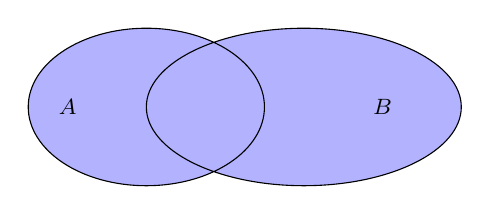
\begin{tikzpicture}[>=stealth,line join=round,line cap=round,font=\footnotesize,scale=1]
	\def\firstellipse{(0.5,0) ellipse (1.5 and 1)}
	\def\secondellipse{(2.5,0) ellipse (2 and 1)}
	\draw[fill=blue!30] \firstellipse \secondellipse;
	%\path (current bounding box.south) node[below=2mm]{$A\cup B$};
	\node at (-0.5,0){$A$};
	\node at (3.5,0){$B$};
\end{tikzpicture}
	\end{center}
	\choice
	{\True $A\cup B$}
	{$A\cap B$}
	{$A\setminus B$}
	{$B\setminus A$}
	\loigiai{
	Phần tô đen trong hình vẽ là hình biểu diễn của tập $A\cup B$.	
	}
\end{ex}

%Câu 10...........................
\begin{ex}%[0T6B3-3]%[Dự án đề kiểm tra NH22-23 - Huỳnh Quy]%[THPT Bình Tân]
	Thống kê số bàn thắng trong các trận đấu tại WORLD CUP 2022 tính đến ngày 20/11/2022 được ghi lại trong bảng tần số sau:
	\begin{center}
	\begin{tabular}{|c|c|c|c|c|c|c|c|c|c|}
	\hline
	Số bàn thắng &$0$ &$1$&$2$&$3$&$4$&$5$&$6$&$7$&$8$\\
	\hline
	Số trận &$5$&$6$&$12$&$5$&$1$&$4$&$1$&$1$&$1$\\
	\hline
	\end{tabular}
	\end{center}
	Mốt của bảng số liệu là
	\choice
	{\True $2$}
	{$12$}
	{$1$}
	{$8$}
	\loigiai{
	Trong bảng số liệu, giá trị $x=2$ có tần số cao nhất nên là mốt của bảng số liệu. 	
	}
\end{ex}

\Closesolutionfile{ans}
%\begin{center}
%	\textbf{ĐÁP ÁN}
%	\inputansbox{10}{ans/ans}	
%\end{center}
\begin{center}
	\textbf{PHẦN 2 - TỰ LUẬN}
\end{center}


%----Câu 1
\begin{bt}%[0T3B1-2]%[Dự án Đề Kiểm tra HKI NH-22-23-TinDatTran]%[THPT Bình Tân]
Tìm tập xác định của hàm số $y=\sqrt{-3x+2}$.
\dapso{$\mathscr{D}=\left(-\infty;\dfrac{2}{3}\right]$ }
\loigiai{
Điều kiện $-3x+2\ge 0 \Leftrightarrow x \le \dfrac{2}{3}$. \\
Vậy tập xác định của hàm số $y=\sqrt{-3x+2}$ là $\mathscr{D}=\left(-\infty;\dfrac{2}{3}\right]$.
}
\end{bt}

%----Câu 2
\begin{bt}%[0T3B2-3]%[Dự án Đề Kiểm tra HKI NH-22-23-TinDatTran]%[THPT Bình Tân]
Vẽ đồ thị hàm số $y=x^2-6x+5$.
\loigiai{
\immini{Đồ thị của hàm số $y=x^2-6x+5$
\begin{itemize}
	\item có tọa độ đỉnh $S\left(3;-4\right)$.
	\item có trục đối xứng là đường thẳng $x=3$.
	\item cắt trục tung tại điểm có tung độ bằng $5$.
	\item cắt trục hoành tại hai điểm có  hoành độ là $x=1$ và $x=5$.
\end{itemize}
Đồ thị hàm số được vẽ như hình bên.}
{
\begin{tikzpicture}[>=stealth,x=1cm,y=1cm,scale=0.8,font=\scriptsize]
\def\a{1} % Hệ số a phải khác 0
\def\b{-6}
\def\c{5}
%\draw[color=gray,dash pattern=on 1pt off 1pt,xstep=1.0cm,ystep=1.0cm] (-5.2,-5.2) grid (5.2,5.2);
\draw[->] (-1,0) -- (7,0) node[below] {$x$};
\draw[->] (0,-5) -- (0,6) node[left] {$y$};
\draw (0,0)node[below left]{$O$};
\draw (3,0)node[above right]{$3$};
\draw (0,-4)node[left]{$-4$};
\node at (5.5,2) [right,font=\footnotesize]{$y=x^2-6x+5$ };
\pgfmathsetmacro\xdinh{-(\b)/2*(\a)}
\pgfmathsetmacro\ydinh{(4*(\a)*(\c)-(\b)^2)/(4*(\a))}
\draw[dashed] (3,5)--(3,-4.5) (0,-4)--(3,-4);
\fill (\xdinh,\ydinh)circle(2pt)node[below right]{$S$};
\clip (-1,-4.5)rectangle(7.5,5.5);
\draw[thick,samples=150,smooth,domain=-5:6.5] plot(\x,{\a*(\x)^2+(\b)*\x+(\c)});
\path (1,0)node[below left]{$1$}  (5,0)node[below right]{$5$} (0,5)node[left]{$5$};
\end{tikzpicture}
}
}
\end{bt}
%----Câu 3
\begin{bt}%[0T5B2-5]%[Dự án Đề Kiểm tra HKI NH-22-23-TinDatTran]%[THPT Bình Tân]
Cho hình chữ nhật $ABCD$ có $AB=5a$, $BC=12a$. Xác định và tính độ dài vectơ
$\left|\overrightarrow{AB}+\overrightarrow{AD}\right|$ theo $a$.
\dapso{$13a$ }
\loigiai{
\begin{center}
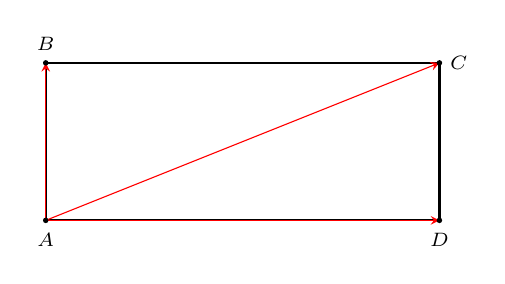
\begin{tikzpicture}[line cap=round,line join=round,scale=1,>=stealth]
\path (0,0) coordinate (A)
(0,2) coordinate (B)
(5,2) coordinate (C)
(5,0) coordinate (D);
\draw [thick] (A)--(B)--(C)--(D)--cycle;
\draw[->,red] (A)--(B); 
\draw[->,red] (A)--(D);
\draw[->,red] (A)--(C);
\foreach \t/\g in {A/-90,B/90,C/0,D/-90}{
\fill (\t) circle (1pt) node[shift={(\g:7pt)},font=\scriptsize]{$ \t $};
}
\end{tikzpicture}
\end{center}
Ta có $|\overrightarrow{AB}+\overrightarrow{AD}|=|\overrightarrow{AC}|=AC=\sqrt{AB^2+BC^2}=\sqrt{(5a)^2+(12a)^2}=13a$.
}
\end{bt}


%----Câu 4
\begin{bt}%[1 điểm]%[0T5K3-4]%[Dự án đề kiểm tra HKI NH22-23-Trương Đăng Khoa]%[THPT Bình Tân]
	Cho tam giác $ABC$. Gọi $I$ là điểm trên cạnh $BC$ sao cho $IC=2IB$. Chứng minh rằng $3\overrightarrow{AI}=2\overrightarrow{AB}+\overrightarrow{AC}$
	\loigiai{
		\begin{center}
			\begin{tikzpicture}
				\path (0,0) coordinate (A)
				(-1,-2) coordinate (B)
				(3,-2) coordinate (C);
				\path ($(C)!2/3!(B)$) coordinate (I);
				\draw [thick,blue] (I)--(A)--(B)--(C)--(A);
				\foreach \t/\g in {A/90,B/180,C/0,I/-90}{
					\draw[fill=white] (\t) circle (1pt) node[shift={(\g:7pt)},font=\scriptsize]{$ \t $};
				}
			\end{tikzpicture}
		\end{center}
		Ta có  $2\overrightarrow{AB}+\overrightarrow{AC}=2(\overrightarrow{AI}+\overrightarrow{IB})+(\overrightarrow{AI}+\overrightarrow{IC})=3\overrightarrow{AI}$, (vì $ 2\overrightarrow{IB}+\overrightarrow{IC}=\overrightarrow{0}$).
	}
\end{bt}

%----Câu 5
\begin{bt}%[1 điểm]%[0T3K2-5]%[Dự án đề kiểm tra HKI NH22-23-Trương Đăng Khoa]%[THPT Bình Tân]
	Trong môn cầu lông, khi phát cầu, người chơi cần đánh cầu \textbf{qua khỏi lưới} sang phía đối phương và \textbf{không} được để cho cầu rơi ngoài biên (\textit{xem hình 10}).\\
	Trong mặt phẳng tọa độ $Oxy$, chọn điểm có tọa độ $(0;y_0)$ là điểm xuất phát thì phương trình quỹ đạo của cầu lông khi rời khỏi vợt là $y=\dfrac{-g\cdot x^2}{2\cdot v_0^2\cdot \cos^2 \alpha}+\tan (\alpha)\cdot x+y_0$; trong đó
	\begin{itemize}
		\item $g$ là gia tốc trọng trường; $\alpha$ là góc phát cầu (so với phương ngang của mặt đất);
		\item $v_0$ là vận tốc ban đầu của cầu; $y_0$ là khoảng cách từ vị trí phát cầu đến mặt đất.
	\end{itemize}
	\begin{center}
		\begin{tikzpicture}[line join=round, line cap=round,scale=1,transform shape]
			\definecolor{beige}{rgb}{0.96, 0.96, 0.86}
			\definecolor{deepskyblue}{rgb}{0.0, 0.75, 1.0}
			\definecolor{battleshipgrey}{rgb}{0.52, 0.52, 0.51}
			\clip (-6,-2) rectangle (7,3.5);
			\tikzset{cau_long/.pic={
					\def\c{
						(-1.32,-.45)
						..controls +(-145:1.4) and +(-125:1.4) ..(-.6,-1.2)
						--cycle
						;}
					\draw[fill=battleshipgrey] \c;
					\draw%[color=battleshipgrey,line width=.5]
					(-1.22,-.35)--(-.5,-1.1)--(1.5,-.2)--(1.8,.22)--(1.2,.16)%1
					--(1.4,.7)--(.8,.6)%2
					--(.9,1.1)--(.4,1)%3
					--(.5,1.5)--(0.05,1.3)%4
					--(.1,1.9)--(-.35,1.65)--cycle
					;
					\draw (1.2,.16)--(-.65,-.92) (.8,.6)--(-.78,-.8) (.4,1)--(-.95,-.62) (0.05,1.3)--(-1.1,-.48) (-.95,.22)--(.1,-.8);
			}}
			%-------------------------------------	
			\draw[dashed] (-3,-0.5)
			..controls +(50:2.3) and +(150:1) .. (3,-1);%đường đi cầu lông
			\draw[dashed] (-3,-0.5)
			..controls +(60:3.3) and +(140:1) .. (4.5,-1);%đường đi cầu lông
			\draw[dashed] (-3,-0.5)
			..controls +(50:4.3) and +(140:1) .. (6.5,-1);%đường đi cầu lông
			%\draw[->](-3,0)--(-2.5,.35);
			%\draw[dashed](-3,0)--(-1.5,0);
			%\node at (-2,0) [above]{\tiny $\alpha =30^\circ$};
			\draw[fill=black] (2.5,-1) circle (1.5pt);
			\node at (3,-1) [below]{\tiny điểm biên trong};
			\draw[fill=black] (6,-1) circle (1.5pt);
			\node at (6,-1) [below]{\tiny điểm biên ngoài};
			\draw[fill=black] (1,-1) circle (1.5pt);
			\node at (1,-1) [below]{\tiny lưới phân cách};
			\node at (1.5,0.2) [below]{\tiny hỏng};
			\node at (2,-1.5) [below]{Hình 10};
			\node at (3.2,0.2) [below]{\tiny hợp lệ};
			\node at (5.2,0.2) [below]{\tiny hỏng};
			\node at (1,-0.5) [left]{\tiny $1{,}524$ m};
			\node at (-1,-1.5) [below]{\tiny $4$ m};
			\draw[<->, line width=2pt] (-3,-1.4)--(1,-1.4);
			%\node at (-.5,-1) [above]{\tiny $y=\dfrac{-g\cdot x^2}{2v_\circ^2\cdot \cos^2\alpha}+\tan (\alpha) \cdot x+y_\circ$};
			\draw[line width=2pt, black] (1,-1)--(1,0);
			\draw (-3,-0.4)pic[scale=.1,rotate=-5]{cau_long};
			
			\def\xmin{-3.5} \def\xmax{7}
			\def\ymin{-1.5} \def\ymax{2} 
			\draw[->] (\xmin,-1)--(\xmax,-1) node [above left]{\tiny $x$};
			\draw[->] (-3,\ymin)--(-3,\ymax) node [left]{\tiny $y$};
			\node at (-3,-1) [below left]{\tiny $O$};
		\end{tikzpicture}
	\end{center}
	Một người đang tập chơi cầu lông, có khuynh hướng phát cầu góc $30^\circ$ (so với mặt đất) biết cầu rời mặt vợt ở độ cao $0,8$ m so với mặt đất và vận tốc xuất phát của cầu là $8$ m/s (bỏ qua sức cản của gió và xem quỹ đạo của cầu luôn nằm trong mặt phẳng thẳng đứng, lấy $g$ là $9,8$ m/s$^2$. Người ấy phát cầu như thế có bị xem là hỏng không? Vì sao? (biết \textit{điểm biên trong} và \textit{biên ngoài} lần lượt cách $O$ là $9,58$ m và $9,94$ m)
	\begin{center}
		\begin{tikzpicture}[line join=round, line cap=round,scale=1,transform shape]
			\definecolor{beige}{rgb}{0.96, 0.96, 0.86}
			\definecolor{deepskyblue}{rgb}{0.0, 0.75, 1.0}
			\definecolor{battleshipgrey}{rgb}{0.52, 0.52, 0.51}
			\clip (-6,-2) rectangle (4,3.5);
			
			\tikzset{cau_long/.pic={
					\def\c{
						(-1.32,-.45)
						..controls +(-145:1.4) and +(-125:1.4) ..(-.6,-1.2)
						--cycle
						;}
					\draw[fill=battleshipgrey] \c;
					\draw%[color=battleshipgrey,line width=.5]
					(-1.22,-.35)--(-.5,-1.1)--(1.5,-.2)--(1.8,.22)--(1.2,.16)%1
					--(1.4,.7)--(.8,.6)%2
					--(.9,1.1)--(.4,1)%3
					--(.5,1.5)--(0.05,1.3)%4
					--(.1,1.9)--(-.35,1.65)--cycle
					;
					\draw (1.2,.16)--(-.65,-.92) (.8,.6)--(-.78,-.8) (.4,1)--(-.95,-.62) (0.05,1.3)--(-1.1,-.48) (-.95,.22)--(.1,-.8);
					
			}}
			
			\draw (-3,0)
			..controls +(50:2.3) and +(150:1) .. (3,-1);%đường đi cầu lông
			\draw[->](-3,0)--(-2.5,.35);
			\draw[dashed](-3,0)--(-1.5,0);
			\node at (-2,0) [above]{\tiny $\alpha =30^\circ$};
			\draw[fill=black] (3,-1) circle (.5pt);
			\node at (3,-1) [below]{\tiny điểm chạm đất};
			\node at (-3,0) [left]{\tiny $y_0=0{,}8$ m};
			\node at (-.5,-1) [above]{\tiny $y=\dfrac{-g\cdot x^2}{2v_\circ^2\cdot \cos^2\alpha}+\tan (\alpha) \cdot x+y_\circ$};
			\path
			(-1.5,.7)pic[scale=.1,rotate=-30]{cau_long};
			
			\def\xmin{-3.5} \def\xmax{4}
			\def\ymin{-1.5} \def\ymax{2} 
			\draw[->] (\xmin,-1)--(\xmax,-1) node [above left]{\tiny $x$};
			\draw[->] (-3,\ymin)--(-3,\ymax) node [left]{\tiny $y$};
			\node at (-3,-1) [below left]{\tiny $O$};
			
			
		\end{tikzpicture}
	\end{center}
	\loigiai{
		Thay $g=9{,}8$ m/s$^2$, góc phát cầu $\alpha=30^\circ$, vận tốc ban đầu $v_0=8$ m/s vào phương trình quỹ đạo của cầu $y=\dfrac{-g\cdot x^2}{2v_0^2 \cdot \cos^2 \alpha}$ ta được $y=-\dfrac{49}{480}x^2+\dfrac{\sqrt{3}}{3}x+0{,}8$.\\
		Xét $y=-\dfrac{49}{480}x^2+\dfrac{\sqrt{3}}{3}x+0{,}8=0$ ta được $x_1\approx 6{,}81$ và $x_2\approx-1{,}15$.\\
		Giá trị nghiệm dương cho ta khoảng cách từ vị trí người chơi cầu lông đến vị trí cầu rơi chạm đất là $6{,}81$ m. Vậy người chơi phát cầu là hỏng vì cầu chạm đất nằm ngoài khoảng biên trong và biên ngoài.
	}
\end{bt}

%----Câu 6
\begin{bt}%[1 điểm]%[0T5K4-3]%[Dự án đề kiểm tra HKI NH22-23-Trương Đăng Khoa]%[THPT Bình Tân]
	Cho tam giác $ABC$ vuông tại $A$ có $AB=a$, $AC=a\sqrt{2}$. Gọi $M$ và $N$ là các điểm thỏa $\overrightarrow{MB}+\overrightarrow{MC}=\overrightarrow{0}$; $\overrightarrow{AN}=2\overrightarrow{BN}$. Chứng minh $AM\perp CN$.
	\dapso{ }
	\loigiai{\immini{
			Ta có $AB\perp AC$ suy ra $\vv{AB}\perp \vv{AC}\Leftrightarrow \vv{AB}\cdot\vv{AC}=0$.\\
			Ta xét
			\begin{eqnarray*}
				\overrightarrow{AM} \cdot \overrightarrow{CN} &=& \dfrac{1}{2}(\overrightarrow{AC} +\overrightarrow{AB}) \cdot (\overrightarrow{CA}+\vv{AN})\\
				&=&\dfrac{1}{2}(\overrightarrow{AC} +\overrightarrow{AB}) \cdot (\overrightarrow{CA}+2\vv{AB})\\
				&=& \dfrac{1}{2}\overrightarrow{AC}\cdot \overrightarrow{CA} + \overrightarrow{AC}\cdot \overrightarrow{AB} + \dfrac{1}{2}\overrightarrow{AB}\cdot \overrightarrow{CA} + \vv{AB}^2\\
				&=& -\dfrac{1}{2}\vv{AC}^2 + \overrightarrow{AC}\cdot \overrightarrow{AB} - \dfrac{1}{2}\overrightarrow{AB}\cdot \overrightarrow{AC} + \vv{AB}^2\\
				&=& -\dfrac{1}{2}AC^2 +\dfrac{1}{2}\vv{AB}\cdot\vv{AC}+AB^2\\
				&=&
				-\dfrac{1}{2}\cdot \left(a\sqrt{2}\right)^2 + 0  +a^2=0.		
			\end{eqnarray*}
			Vậy $\vv{AM}\perp \vv{CN}$ hay $AM\perp CN $.
		}{\begin{tikzpicture}
				\path (0,0) coordinate (A)
				(3,0) coordinate (B)
				(0,4.24) coordinate (C);
				\path ($(C)!0.5!(B)$) coordinate (M)
				($(A)!2!(B)$) coordinate (N);
				\path (intersection of A--M and C--N) coordinate (I);
				\path pic[draw,angle radius=5pt]{right angle= A--I--N};
				\draw (C)--(N) (A)--(I) (B)--(N);
				\draw [thick,blue] (A)--(B)--(C)--cycle;
				\foreach \t/\g in {A/180,B/-90,C/90,M/15,N/-90,I/15}{
					\draw[fill=white] (\t) circle (1pt) node[shift={(\g:7pt)},font=\scriptsize]{$ \t $};
				}
	\end{tikzpicture}}}
\end{bt}












